\chapter{Sekwencjonowanie i adnotacja genomu}
\label{section:biologiny_wstep}

\section{Sekwencjonowanie i asembling DNA}
Sekwencjonowanie to jedna z technik biologii molekularnej, pozwalająca na odczytanie kolejności nukleotydów w cząsteczce DNA.

Najlepiej byłoby, gdyby projekt genomu reprezentował kompletną sekwencję nukleotydową wszystkich chromosomów danego gatunku. 
Jednak w rzeczywistości, istnieje wiele potencjalnych problemów związanych z procesem sekwencjonowania. Nie istnieje bowiem, jedna, prawdziwa sekwencja dla gatunku z powodu indywidualnej zmienności genetycznej jednostek. 
Nawet komórki tego samego osobnika mogą różnić się w zawartości genetycznej z powodu mutacji somatycznych. Złożony genom będzie tylko jedną reprezentacją wariacji występującej u danego gatunku. 
Zasadniczo sekwencjonuje się tylko jednego osobnika, ale czasami genom stanowi konsensus wielu połączonych próbek (projekt HUGO). 
Należy zdawać sobie sprawę, że procesowi sekwencjonowania zawsze będą towarzyszyć błędy na poziomie poszczególnych nukleotydów oraz ich kolejności (błędy montażu). 
Każdy złożony genom jest wynikiem serii złożeń metodami heurystycznymi i powinien być traktowany jako robocza hipoteza.

\begin{figure}[h]
	\centering
	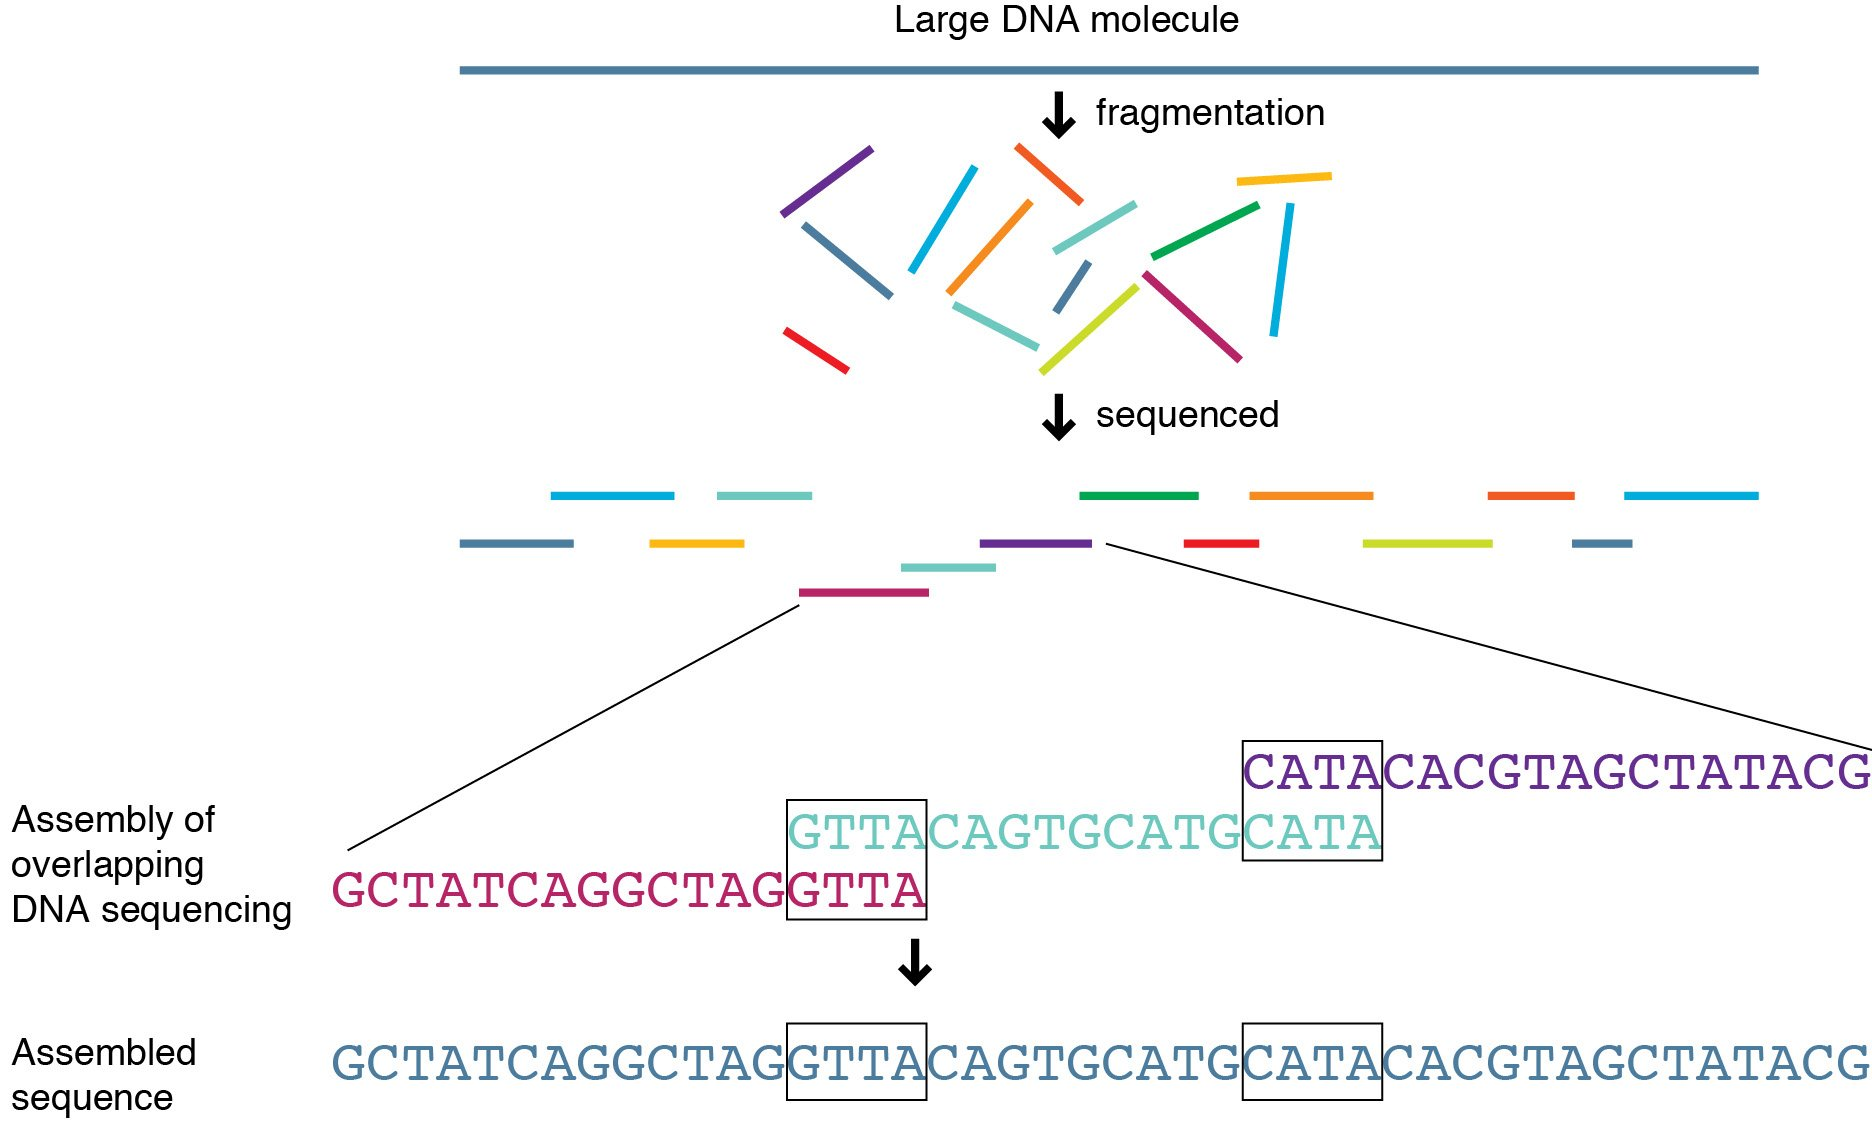
\includegraphics[width=0.9\textwidth]{img/sequenctioning-process.png}
	%zdjecie z %http://knowgenetics.org/whole-genome-sequencing/
	\caption{Schemat sekwencjonowania}
	\vspace{-0.5cm}
	\caption*{\scriptsize Źródło: \url{http://knowgenetics.org/whole-genome-sequencing/}}
	\label{img:schemat-sekwencjonowania}
\end{figure}

Większość projektów, w początkowej fazie sekwencjonowania kieruje się strategią polegającą na losowym pocięciu DNA na bardzo małe fragmenty.
W zależności od wykorzystanej technologii, fragmenty mogą mieć różne długości. Istnieje trend w kierunku przeprowadzania odczytów technikami dającymi coraz krótsze fragmenty. 
Tradycyjne sposoby (Sanger) dawały fragmenty długości około 1000 par zasad. Obecnie wykorzystywane techniki dające najkrótsze rezultaty osiągają wyniki rzędu dziesiątek pz. (SOLiD, Illumina - rys.\ref{img:sekwencjoner-illumina}).

\begin{figure}[h]
	\centering
	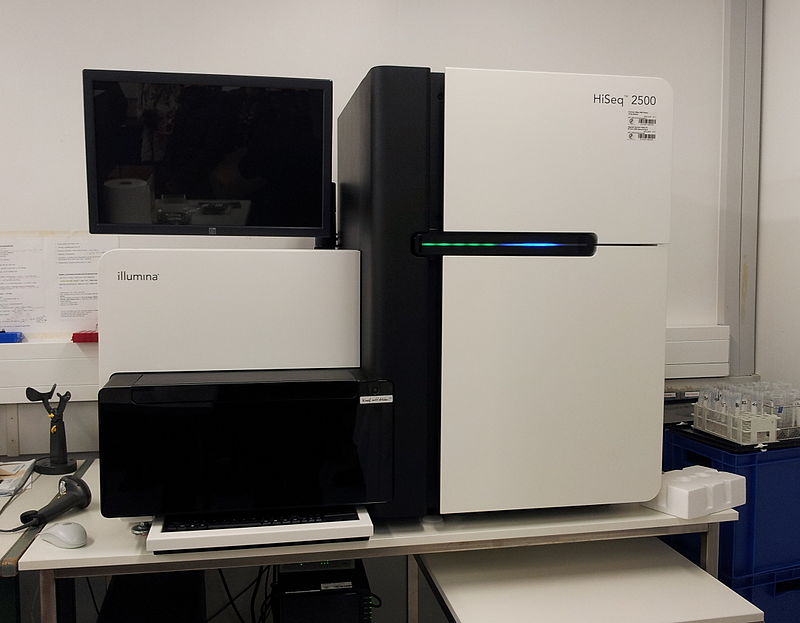
\includegraphics[width=0.75\textwidth]{img/sekwencjoner-illumina.jpg}
	%zdjecie z http://wiedza.alkahest.umcs.pl/jak-limfocyty-t-przekazuja-informacje/
	\caption{Sekwencjoner Illumina HiSeq 2500}
	\vspace{-0.5cm}
	\caption*{\scriptsize Źródło: \url{http://wiedza.alkahest.umcs.pl/jak-limfocyty-t-przekazuja-informacje/}}
	\label{img:sekwencjoner-illumina}
\end{figure}

Następie, w procesie asemblingu, fragmenty sekwencji są składane w dłuższe odcinki. Dobór algorytmu jest zależny od długości odcinków zsekwencjonowanych w poprzednim etapie. Jest to proces skomplikowany i wykorzystywane są do tego zasobożerne programy. 
Efektem początkowego składania sekwencji są kontigi.
Na dalszych etapach, po analizach wykorzystujących biblioteki dłużych sekwencji DNA, kontigi są zespalane w struktury zwane skafoldami.
Mają one zazwyczaj postać sekwencji z lukami o znanej długości - dziury oznaczane są znakiem ,,N''.

\section{Adnotacje}
Aby wykorzystać cały potencjał sekwencji genomu, musi on zostać opatrzony adnotacjami, które zawierają istotne informacje z biologicznego punktu widzenia. Kompletna adnotacja genomu stanowi duże wyzwanie dla biologów, a jej wyniki są w dużej mierze uzależnione od jakości złożenia genomu w procesie asemblingu.

Adnotacja genomu jest procesem odnalezienia regionów kodujących, zidentyfikowania genów oraz określenia funkcji jakie pełnią. Adnotacją możemy nazywać np. przypis będący notatką dodaną jako wyjaśnienie bądź komentarz. Dzielą się na przypisy:
\itemize{
	\item strukturalne (identyfikacja obiektów genomowych)
	\item funkcjonalne (biologiczne informacje związane z obiektami genomowymi)
}
\\
Proces adnotacji można podzielić na 3 główne fazy:
\enumerate{
	\item Identyfikacja niekodujących fragmentów.
	\item Przewidywanie genów.
	\item Dołączenie biologicznych informacji.
}\\

Większość technik wykorzystuje narzędzia oparte o wyszukiwanie homologicznych sekwencji używając do tego celu publiczne bazy danych genomów. Przewidywanie genów to czynność mająca na celu zidentyfikowanie fragmentów DNA, które odpowiedzialne są za kodowanie białek. Wśród organizmów zbudowanych z komórek posiadających jądro komórkowe z chromosomami (eukarioty), odcinki kodujące sekwencję aminokwasów nazywane są eksonami, które zazyczaj oddzielone są fragmentami niekodującymi - intronami (rys.\ref{img:intron-exon}).

\begin{figure}[h]
	\centering
	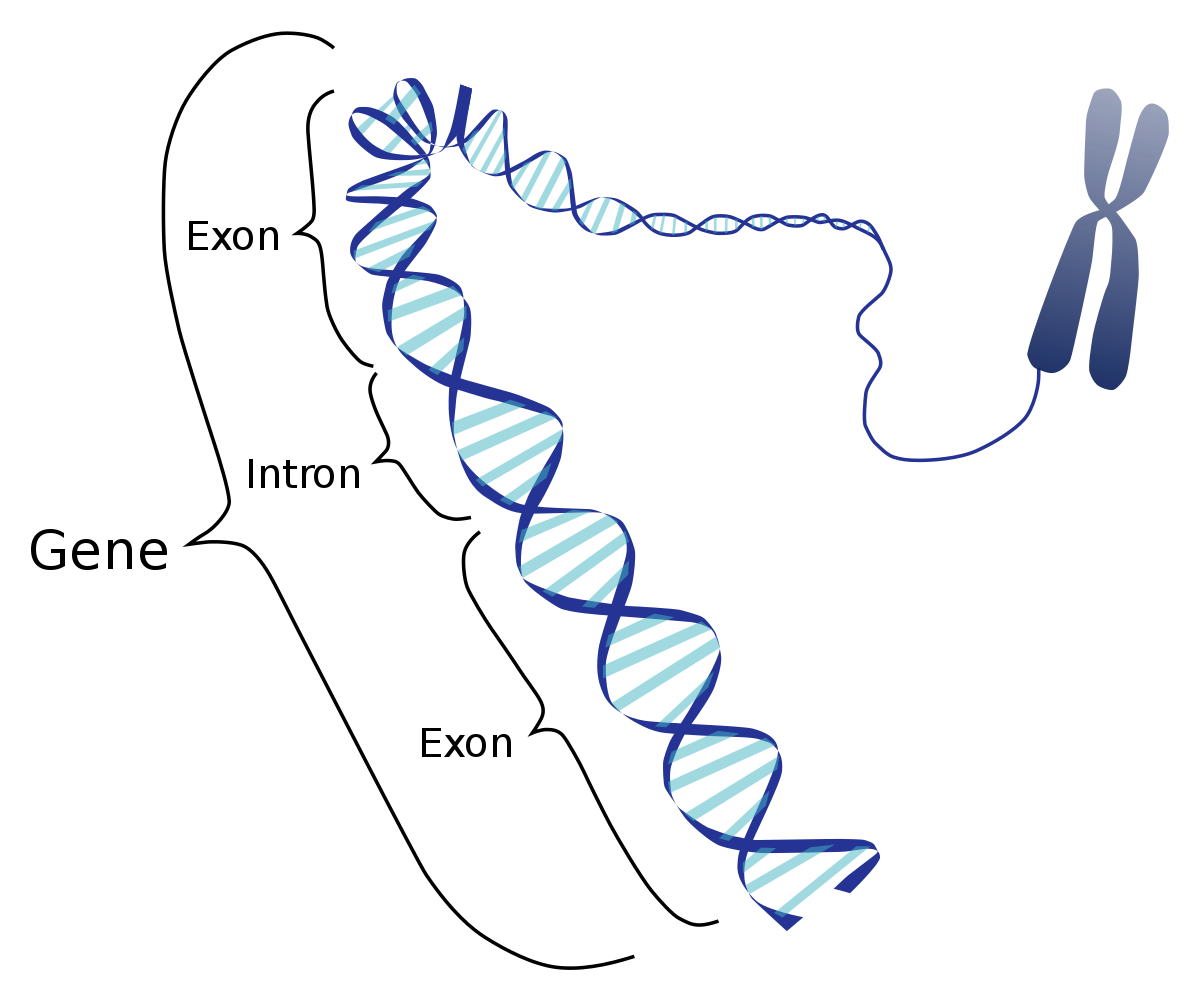
\includegraphics[width=0.75\textwidth]{img/intron-exon.png}
	\caption{Reprezentacja intronów i eksonów z genem zawierającym pojedynczy intron i dwa eksony.}
	\vspace{-0.5cm}
	\caption*{\scriptsize Źródło: \url{https://en.wikipedia.org/wiki/File:Gene\_Intron\_Exon\_nb.svg}}
	\label{img:intron-exon}
\end{figure}


\section{Prezentacja danych}
Kolejnym etapem projektu poznania genomu jest zazwyczaj umieszczenie go w przeglądarce genomów wraz z adnotacjami. Są to programy mające wygodny interfejs graficzny, gromadzące i w przystępny sposób prezentujące informacje uzyskane w poprzednich etapach badań. Dzięki nim naukowcy mają możliwość przede wszystkim łatwego dostęp do danych, a także posiadają wygodne narzędzie do dalszych prac. 
Ważnym aspektem jest fakt, że dzięki przeglądarkom mogą dzielić się wynikami prac z innymi zespołami badawczymi, bez czego postęp biotechnologiczny rozwijałby się znacznie wolniej.

Dane wizualizowane są najczęściej w sposób interaktywny pozwalając na obserwację genomu z perspektyw makro (chromosomów) i mikro (poszczególne geny, ciągi nukleotydowe).


\section{Przegląd literatury - istniejące rozwiązania}
\begin{itemize}
	% https://en.wikipedia.org/wiki/UCSC_Genome_Browser
	% http://genome.ucsc.edu/
	\item \href{https://genome.ucsc.edu}{\emph{UCSC browser}} \label{przegladarka-UCSC}\\
	przeglądarka on-line, opracowana na Uniwersytecie Kalifornijskim w~Santa Cruz w 2000 roku; główni autorzy - Jim Kent, David Haussler; zaimplementowana w~większości w~języku~C. Udostępniana darmowo dla akademickich zastosowań, dla komercyjnych wymagana licencja \emph{Kent Informatics}. Zawiera 46 gatunków organizmów. Pozwala wyświetlać sekwencje o dowolnym rozmiarze - od pojedynczych zasad po chromosomy. Badacze mogą wyświetlać własne dane i wyświetlać je w kontekście referencyjnego genomu. Widoki tworzone przez użytkowników mogą być udostępniane innym użytkownikom.
	
	W porównaniu do CuGene:
	brak możliwości wyprodukowania fragmentów genomu z priorytetyzacją nakładających się na siebie typów danych. Brak algorytmów wyszukiwania Knutha-Morrisa-Pratta i Smitha-Watermana. Skomplikowane narzędzie, trudne dla początkujących użytkowników.
	
	\begin{figure}[h]
		% https://en.wikipedia.org/wiki/UCSC_Genome_Browser#/media/File:BrowserFoxp2.jpg
		\centering
		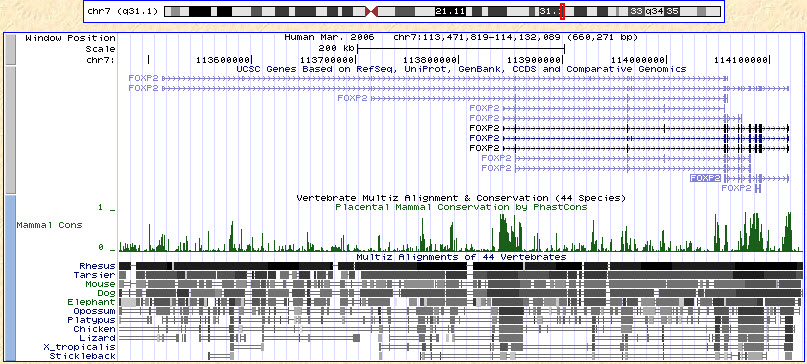
\includegraphics[width=0.75\textwidth]{img/browser-UCSC.jpg}
		\caption{Przeglądarka UCSC.}
		\vspace{-0.5cm}
		\caption*{\scriptsize Źródło: \url{https://en.wikipedia.org/wiki/UCSC\_Genome\_Browser\#/media/File:BrowserFoxp2.jpg}}
		\label{img:przegladarka-UCSC}
	\end{figure}
	
	
	\item \href{http://gbrowse.org}{\emph{Gbrowse}} - \label{Gbrowse}
	największa część kodu to Perl, z~czasem coraz więcej JavaScriptu. Prace rozpoczęto w~2002 roku, funkcjonuje na licencji \emph{PERL artistic license}. %\cite{pdf-mimuw}
	
	\item \href{http://www.ensembl.org}{\emph{ENSEMBL}} \label{ENSEMBL}
	- funkcjonuje na licencji Apache, dopuszczającej użycie kodu źródłowego zarówno na potrzeby wolnego oprogramowania, jak i~zamkniętego oprogramowania komercyjnego. Znaczna część kodu napisana w~Perlu, schemat bazy danych w~MySQl. %\cite{pdf-mimuw, pl-wiki-apache}
	
	\item \href{http://bioviz.org/igb/index.html}{\emph{Integrated Genome Browser}} \label{IGB}
	- projekt rozpoczęty przez firmę \emph{Affymetrix}, jednak porzucony przez nią i~rozwijany w~środowisku akademickim. Przeglądarka napisana w~Javie, obecnie na prawach Academic free license. %\cite{pdf-mimuw}
	
	\item \href{http://www.interactive-biosoftware.com/alamut-visual/features/}{\emph{Alamut}} \label{alamut}- przeglądarka z~prostym interfejsem użytkownika z~adnotacjami pobieranymi z~publicznie dostępnych baz NCBI, EBI, UCSC. Zgodna z~nomenklaturą HGVS (ang. \emph{Human Genome Variation Society}). Funkcjonalność obliczeniowa oparta o~narzędzia predykcyjne.
	
	\item \href{http://www.broadinstitute.org/annotation/argo/}{\emph{Argo Genome Browser}} \label{argo-genome-browser}- narzędzie służące do wizualizacji i~manualnego dodawania adnotacji genomów. Oprogramowanie open-source na licencji LGPL, napisane w~języku \emph{Java}.
	
	\item \href{http://www.bioinformatics.babraham.ac.uk/projects/chipmonk/}{\emph{ChIPMonk}} \label{chipmonk}- narzędzie opracowane w~Instytucie Babraham Cambridge, służy do obrazowania i~analizy tablic danych \emph{ChIP-on-chip}. Kod wydany na licencji GPL v2. Projekt przestał być rozwijany.
	
	\item \href{http://www.biodalliance.org/}{\emph{Biodalliance}} \label{biodalliance} - szybka, interaktywna wizualizacja genomów w~przeglądarce internetowej. Oparta o~\emph{JavaScript}, wspiera wiele najpopularniejszych formatów danych genetycznych. Rozwiązanie łatwe do wbudowania we własne aplikacje czy strony internetowe.
	
	\item \href{https://www.dnanexus.com/genomes/hg18/public_browse}{\emph{DNAnexus}} \label{dnanexus} - przeglądarka do wizualizacji danych korzysta z~technologii \emph{Flash}. Jest narzędziem nowej generacji, mocno rozbudowanym w~kategorii analizy i~obrazowania sekwencji.
	
	\item \href{http://download.cnet.com/GeneWall-Genome-Browser-Pro/3000-2129_4-75855506.html}{\emph{GeneWall}} \label{genewall} - przeglądarka genomów przeznaczona na urządzenia mobilne. W~wersji podstawowej można przeglądać jedynie genom człowieka, natomiast w~wariancie profesjonalnym aplikacji mamy możliwość uploadu własnych plików z~danymi.
	
	\item \href{http://gaggle.systemsbiology.net/docs/geese/genomebrowser/}{\emph{Gaggle Genome Browser}} \label{gaggle} - otwarte narzędzie do mapowania mocno skondensowanych danych na współrzędne genomu. Oprogramowanie przeznaczone do obsługi dużych zbiorów danych, pozwala na łatwy import plików użytkownika. Współpracuje z~innymi bioinformatycznymi narzędziami zawartymi w~frameworku Gaggle.
	
	\item \href{https://genestack.com/}{\emph{Genestack}} \label{genestack} - internetowy, genomiczny system operacyjny. Pozwala wyszukiwać i~importować dane z~wielu publicznych baz danych. Potrafi konwertować dane wejściowe użytkowników z~wielu formatów. Udostępnia zestaw narzędzi dla programistów, do łatwego tworzenia własnych przeglądarek.
	
	\item \href{http://genomeview.org/}{\emph{GenomeView}} \label{genomeview} - samodzielna przeglądarka i~edytor genomu nowej generacji. Obecnie rozwijana przez społeczność \href{http://www.broadinstitute.org/}{Broad Insitute}. Zapewnia interaktywną wizualizację sekwencji, adnotacji, możliwość porównań na wielu poziomach, mapowań i~wielu innych. Dzięki systemowi wtyczek, istnieje możliwość rozszerzenia funkcjonalności przeglądarki.
	
	\item \href{http://www.genomemaps.org/}{\emph{GenomeMaps}} \label{genomemaps} - wysokowydajna przeglądarka z~interfejsem opartym o~HTML5 i~CSS3. W~dużej mierze implementowana z~użyciem biblioteki Javascript \href{https://github.com/opencb/jsorolla}{\mbox{\emph{JSorolla}}}. Dane pozyskuje korzystając z~usług REST bazy \href{https://github.com/opencb/cellbase/wiki}{\emph{CellBase}}. Uruchamia się we wszystkich nowszych przeglądarkach internetowych, nie wymagając od użytkownika instalacji dodatkowych komponentów.
	
	\item \href{http://www.popsci.com/science/article/2011-06/introducing-genome-wowser-ipad-app-lets-you-browse-human-genome}{\emph{Genome Wowser}} - aplikacja przeznaczona na urządzenia mobilne iPad, wydana przez CBMI (ang. Center for Biomedical Informatics) w~Szpitalu Dziecięcym w~Filadelfii. Pozwala przeglądać popularną bazę \emph{UCSC Genome Browser}.
	
	\item \href{https://hyperbrowser.uio.no/hb/}{\emph{Genomic HyperBrowser}} - jest wolnym oprogramowaniem na licencji \emph{GNU GPL v3}. Produkt skupiony głownie na analizie statystycznej elementów w~genomie. Tworzony z~wykorzystaniem platformy \href{https://en.wikipedia.org/wiki/Galaxy_(computational_biology)}{\emph{Galaxy}}.
	
	\item \href{http://wtsi-web.github.io/Genoverse/}{\emph{Genoverse}} - przenośna, konfigurowalna, przeglądarka oparta o~Javasript i~HTML5. Pozwala na eksplorację danych w~dynamiczny, interaktywny sposób. Dane są prezentowane w~przeglądarce, dzięki czemu może być łatwo instalowana na własnych stronach i~pokazywać dane z~wielu źródeł - gromadzonych online i~lokalnie.
	
	\item \href{http://genplay.einstein.yu.edu/}{\emph{GenPlay}} - szybkie i~łatwe w~użyciu narzędzie do analizy i~przetwarzania sekwencji napisane w~Javie. Uruchamia się na większości najpopularniejszych systemów operacyjnych. Prace nad projektem rozpoczęto na Kolegium Medycznym Alberta Einstein'a Uniwersytetu Yeshiva w~Nowym Yorku. Przeglądarka aktualnie w~fazie testowania, używana przez studentów.
	
	\item \href{http://img.jgi.doe.gov/}{\emph{Integrated Microbial Genomes}} - zaawansowany system wspierający analizę i~adnotacje mikrobiologicznych zbiorów danych i~metadanych genetycznych zgromadzonych w~\emph{DOE's Joint Genome Institute}. Współpracuje z~wieloma instytucjami.
	
	\item \href{http://mgv2.cmbi.ru.nl/}{\emph{Microbial Genomic Viewer}} - łatwe w~obsłudze narzędzie do interaktywnej wizualizacji wyników analizy porównawczej genomów. 
	
	\item \href{https://www.nextbio.com}{\emph{NextBio Genome Browser}} - interaktywna aplikacja pozwalająca na wizualizację zależności pomiędzy prywatnymi lub publicznymi zbiorami danych biologicznych różnych typów.
	
	\item \href{http://persephone.net/}{\emph{Persephone}} - rozbudowana aplikacja nowej generacji szeroko używana przez bioinformatyków i~genetyków. Możliwość bezpłatnego korzystania z~wersji \emph{trial} przez 30 dni.
	
	\item \href{http://www.plantgdb.org/}{\emph{PlantGDB}} - przeglądarka z~zestawem narzędzi analitycznych wraz ze zbiorami danych genetycznych wielu roślin.
	
	\item \href{http://tabit.ucsd.edu/}{\emph{STAR}} - zintegrowane środowisko do zarządzania i~wizualizacji danych sekwencjonowania. Płynność działania aplikacji w~przeglądarce internetowej zapewnia połączenie technologi JavaScript, HTML5 i~asynchronicznej komunikacji do wymiany danych. 
	
	\item \href{http://tgac-browser.tgac.ac.uk/}{\emph{TGAC Browser}} - nowa open-source'owa przeglądarka genomów obrazująca adnotacje z~bazy danych \emph{Ensembl}. Wyprodukowana przez \emph{Centrum Analizy Genomów} w~Wielkiej Brytanii (ang.\emph{The Genome Analysis Centre, UK}).
	
	\item \href{http://ugene.net/}{\emph{Ugene}} - darmowa platforma bioinformatyczna wspomagająca użytkowników w~pracach nad sekwencjami. Oferuje narzędzia do analizy danych, przypisów, porównań itp. Dane wejściowe mogą być składowane lokalnie albo udostępnione z~innych źródeł. Napisana w~C++ z~wykorzystaniem biblioteki Qt. Funkcjonuje na licencji GPL.
	
	\item \href{http://enhancer.lbl.gov/}{\emph{VISTA Enhancer Browser}} - kompleksowy zestaw baz danych, narzędzi, serwerów na potrzeby analizy porównawczej sekwencji genomów. Istnieją 2 sposoby na korzystanie z~przeglądarki: można wysyłać własne sekwencje i~dopasowania do analizy, bądź sprawdzać z~wstępnie przetworzonymi danymi całych genomów różnych gatunków. Projekt rozwijany we współpracy z~wieloma instytucjami.
	
	
\end{itemize}